\documentclass[twoside]{article}

% AISTATS 2027 submission, anonymous.
\usepackage{aistats2027}
\usepackage{graphicx}
\usepackage{amsmath,amssymb}
\usepackage{booktabs}
\usepackage{microtype}
\usepackage[round]{natbib}

\bibliographystyle{apalike}

\begin{document}

\twocolumn[
\aistatstitle{SPARC: Calibrated Day-Ahead Electricity Price-Spread Intervals from Binding-Constraint Attention}
\aistatsauthor{Anonymous}
\aistatsaddress{Anonymous submission}
]

\begin{abstract}
Nodal power hedging is a bet on the spread between two grid locations, so traders need a calibrated predictive distribution rather than a point forecast. Most day-ahead price models are scored on mean error and treat locational prices as generic time series, leaving the hedging interval untested and the market-clearing constraints unread. We propose SPARC (\textbf{C}onstraint-\textbf{A}ware \textbf{S}pread \textbf{P}redictor), which forecasts the ERCOT day-ahead spread from binding constraints and shadow prices published at the previous day's clearing. Attention over constraint slots learns how much each binding line moves the source-sink path, and the model runs on CPU with under nine thousand trainable parameters. Across a broad baseline suite, SPARC gives the best-calibrated central interval. Its empirical coverage reaches 89.4\% at the requested level, while linear quantile regression reaches 73.1\% despite lower average quantile error. Removing attention costs 11.9 coverage points with little change in mean error. A calendar-year transfer test retains the coverage edge, and the results expose a metric paradox: calibrated intervals favor SPARC, average quantile loss favors the linear model, and the winner depends on the decision metric.
\end{abstract}

\section{Introduction}
A nodal power hedge is a bet on the price difference between two locations, not on the system price itself. A market participant who buys at a hub and sells at a load pocket, or who prices a financial transmission right against an expected congestion corridor, needs the full predictive distribution of that spread. The position size is not a median forecast; it is a quantile of the loss distribution, because a band that promises ninety percent coverage but delivers seventy-three percent leaves the desk systematically under-hedged \citep{bessa2017improved}. This makes probabilistic calibration a decision-relevant property, not a secondary evaluation ritual.

Two gaps separate the standard forecasting pipeline from that decision. First, electricity-price research has historically scored point accuracy, so the interval a trader actually uses is often not the object under comparison \citep{lago2020forecasting, hong2020energy}. Probabilistic price forecasting has improved, but many evaluations still reward sharpness without penalizing the width-aware violation cost that a hedging desk pays \citep{gneiting2007strictly, bracher2021evaluating}. Second, most day-ahead locational-price models treat the price as a generic temporal signal, using lags, calendar features, weather, load, or cross-market prices \citep{toubeau2020capturing, das2021forecasting}. They ignore the mechanism that actually moves a nodal spread: the binding constraints and shadow prices published at every market clearing. This is a missed input, because locational marginal prices decompose into a system energy term plus a congestion component, and the spread between two nodes cancels the common energy term, leaving a congestion residual \citep{hong2020locational}.

We propose SPARC, a compact constraint-attention network for day-ahead ERCOT spread intervals. The key idea is output-conditioning: when the target is downstream of a published market optimization, read the optimizer's own outputs. SPARC takes the top binding constraints by shadow price from the previous day's clearing, encodes each as a short feature slot, and learns how much each constraint moves the source-sink path through attention. This differs from formula embedding, which hard-codes a known settlement rule into the architecture \citep{yu2026marketruleinformed}. ERCOT does not expose the relevant shift factors in closed form at bid time, so SPARC conditions on the published primal and dual outputs instead of assuming a functional form. The model is deliberately small, 8{,}978 trainable parameters, and runs on commodity CPU, which matches the practical cadence of a desk that retrains on a recent rolling window.

The evidence shows a sharp split in model rankings. SPARC achieves the best-calibrated central band and the best width-aware interval score in a broad baseline comparison, while linear quantile regression achieves lower average quantile loss and tighter point error. The decomposition is diagnostic: removing attention leaves mean error almost unchanged, but approximately removes the calibration advantage, indicating that the gain comes from how constraints are weighted rather than from added capacity. This exposes a metric paradox. Average quantile loss and calibrated-interval evaluation answer different questions, and they disagree on the best model. Since a position sized from quantiles incurs a direct penalty for interval violations, the width-aware score is the decision metric \citep{hobbs2022probabilistic}.

Our contributions are three. First, an output-conditioned forecaster: SPARC predicts the day-ahead spread from the market clearing's published constraint outputs, with attention learning endogenous exposure weights over the source-sink path. Second, a calibration-first result: across twelve baselines, including classical, tree-based, and deep models, SPARC gives the highest empirical coverage and the best width-aware interval score at a small CPU-scale parameter budget. Third, a documented metric paradox: we report both average quantile loss and interval calibration and show that the preferred model depends on which decision metric is used, with implications for how probabilistic price forecasters should be evaluated.

The rest of the paper places this work in the literature, derives the spread identity, describes the constraint-attention architecture, presents the main results and ablations, tests rival fusions, and concludes with limitations and future directions.

\section{Related Work}

\subsection{Electricity Price Forecasting}
Electricity-price forecasting has been dominated by point-error benchmarks, with autoregressive and expert models serving as strong baselines \citep{lago2020forecasting, uniejewski2018efficient}. The day-ahead setting is unusually competitive: linear and shrinkage models frequently outperform larger neural networks on average error because the price series is noisy and nonstationary \citep{lago2020forecasting}. Deep probabilistic models have nevertheless become standard, including quantile recurrent networks, distributional neural networks, and attention-based hybrids \citep{wen2017multihorizon, marcjasz2023distributional, lim2020temporal}. These models typically condition on the price's own history and a set of market-wide covariates, without a direct representation of the network constraints that create locational price differences. Our work does not compete on point-error capacity. It competes on the identification of the input that moves the spread, which the classical price-series paradigm leaves out.

\subsection{Market-Rule-Informed and Locational-Price Models}
Locational marginal price theory explains why the spread is a natural target for structured forecasting \citep{hong2020locational}. Several papers have moved beyond scalar system prices and studied either day-ahead to real-time price differences or distribution-locational-price uncertainty \citep{das2021forecasting, toubeau2020capturing}. These models improve over generic series by capturing spatiotemporal market structure, but they still learn it from prices rather than from the clearing's constraint outputs. The closest lineage is market-rule-informed learning. Yu et al.\ embed a settlement formula into a neural network for imbalance prices, treating the known rule as a differentiable structural prior \citep{yu2026marketruleinformed}. SPARC takes the complementary route. Where formula embedding assumes the functional relationship between prices and congestion, output-conditioning reads the primal and dual solution actually published by the clearing. This matters for ERCOT, where shift factors are endogenous to dispatch and no clean closed form is available at bid time. In SPARC, the model learns exposure endogenously through attention, which is a different inductive bias from hard-coded formula layers.

\subsection{Probabilistic Calibration and Decision-Aligned Evaluation}
Probabilistic forecasting research has developed interval-specific evaluation, proper scoring rules, and calibration diagnostics \citep{gneiting2007strictly, bracher2021evaluating}. Quantile regression remains a central tool in energy applications \citep{taieb2016forecasting}, and conformal methods can provide finite-sample coverage under exchangeability \citep{vovk2005algorithmic, lei2018distribution}. A recurring challenge is quantile crossing, addressed by non-crossing constraints, isotonic post-processing, or hierarchical quantile models \citep{chen2025outlieradaptivebased, taieb2020hierarchical}. SPARC combines a soft quantile head with a training-time coherence penalty, and reports a hierarchical variant that enforces ordering by construction. The larger issue is metric selection. Different proper scoring rules reward different properties, and the interval score is explicitly connected to the cost borne by a decision maker whose position depends on the band \citep{bracher2021evaluating, hobbs2022probabilistic}. This line of work supports the paper's central framing: calibration at the hedging interval, not average quantile error, is the property that matters for price-spread risk sizing.

\section{Background and the Old View}
A day-ahead locational marginal price at settlement point $i$ decomposes into a system energy term and a congestion term,
\begin{equation}
\mathrm{LMP}_{i,t} = \lambda_t + \sum_{k} \mathrm{SF}_{k,i,t}\,\mu_{k,t},
\end{equation}
where $\lambda_t$ is the system energy price, $\mathrm{SF}_{k,i,t}$ is the shift factor of point $i$ on constraint $k$, and $\mu_{k,t}$ is the shadow price. The spread between two points cancels the common energy term, leaving a congestion differential. This is why the published binding constraints and their shadow prices are the natural inputs.

The market clears once per day, for all 24 delivery hours, in a single security-constrained unit commitment and economic dispatch run. At bid time for delivery hour $t$ of day $D$, the most recent completed clearing is the previous day's, and the freshest snapshot for hour $t$ is the same hour one day earlier. The model therefore uses a 24\,h lead. A shorter lead would sit inside the same auction as the target and would not be available when the bid is placed.

The standard view treats the spread as a generic time series. Quantile regression on the spread's own history and generic covariates already outputs quantiles, so the gap is not point versus quantile. The gap is inputs. Such models never read the published constraints, so they cannot condition on the mechanism that moves the spread, and they go miscalibrated when congestion binds.

\section{Method}
We denote the day-ahead spread at delivery hour $t$ by
\begin{equation}
s_t = \mathrm{LMP}_{i,t} - \mathrm{LMP}_{j,t},
\end{equation}
where $i$ is the source node and $j$ is the sink node. At bid time for hour $t$, the freshest published clearing is the hour $t-24$ snapshot. That snapshot contains the set of binding transmission constraints, each with a shadow price $\mu_k$, a constraint identifier, the voltage level of the constrained element, and a flow ratio. We keep the top $K=50$ constraints by shadow-price magnitude and encode each as a four-dimensional slot
\begin{equation}
x_k = \left[\,\mu_k,\; \mathrm{id}_k,\; \mathrm{kV}_k,\; \min(r_k,5)\,\right],
\end{equation}
where the flow ratio is clipped to $[0,5]$ to prevent rare extreme values from dominating the slot representation. Slots are zero-padded when fewer than $K$ constraints bind, and no learned no-congestion embedding is used.

The input choice follows directly from the locational-price identity
\begin{equation}
\mathrm{LMP}_i - \mathrm{LMP}_j
= \sum_{k} \left( \mathrm{SF}_{k,i} - \mathrm{SF}_{k,j} \right) \mu_k,
\end{equation}
which holds because the common system energy term cancels in the difference. ERCOT does not publish bid-time shift factors in a closed form that can be inserted into the model, so SPARC does not hard-code the functional relationship. Instead, it conditions on the clearing outputs, which are the primal and dual variables of the same optimization that produced the spread. This is the core distinction from formula-embedding methods such as MRINN, where a known settlement rule is embedded as a differentiable structural prior \citep{yu2026marketruleinformed}. SPARC learns the exposure weights endogenously.

The slot encoder applies a shared linear map from the four slot features to an eight-dimensional embedding,
\begin{equation}
e_k = W_s x_k + b_s,
\qquad W_s \in \mathbb{R}^{8 \times 4}.
\end{equation}
A source-sink pair embedding $z_p$ captures the identity of the corridor being priced, and an eighteen-dimensional temporal vector $h_t$ carries six Fourier terms for hour of day and day of week, together with the lagged spreads $s_{t-24}$, $s_{t-48}$, and $s_{t-168}$. The temporal branch is deliberately small; it supplies calendar and recent-price context, while the constraint branch carries the congestion signal.

The constraint view is computed by attention over the encoded slots. The query is derived from the pair embedding only,
\begin{equation}
q = W_q z_p,
\qquad q \in \mathbb{R}^{8},
\end{equation}
and the slot keys are the encoded slot vectors $e_k$. The attention weights are
\begin{equation}
a_k = \frac{\exp\!\bigl( q^\top e_k / \sqrt{8} \bigr)}
{\sum_{\ell=1}^{K} \exp\!\bigl( q^\top e_\ell / \sqrt{8} \bigr)}.
\end{equation}
Each slot also emits a scalar shadow-price readout $\tilde{\mu}_k = w_m^\top e_k$, so that the attended congestion view is
\begin{equation}
c = \sum_{k=1}^{K} a_k \, \tilde{\mu}_k.
\end{equation}
This operation is permutation invariant over the unordered constraint set, and it yields a scalar that can be interpreted as a learned path exposure times shadow price. The pair-embedding query lets the same slot set produce different congestion views for different source-sink corridors, which is necessary because each pair has its own shift-factor differentials.

The head concatenates the pair embedding, temporal vector, and attended congestion view, $z = [\,z_p\,;\,h_t\,;\,c\,]$, and passes $z$ through a multi-layer perceptron with hidden width 128. The output layer emits the seven quantiles $\hat q^{0.10}, \hat q^{0.25}, \hat q^{0.45}, \hat q^{0.50}, \hat q^{0.55}, \hat q^{0.75}, \hat q^{0.90}$.

The flagship SPARC head uses a soft quantile layer. As a coherence-by-construction alternative, we also train a hierarchical head that outputs a median and adds nonnegative softplus increments outward. Because the increments are nonnegative, the hierarchical head produces ordered quantiles without a penalty term.

Training minimizes the quantile loss over all seven levels. For a target $y$ and a quantile estimate $\hat q^\tau$, the pinball loss is
\begin{equation}
\rho_\tau(y - \hat q^\tau)
= (y - \hat q^\tau)\left( \tau - \mathbf{1}[y < \hat q^\tau] \right),
\end{equation}
and the full objective is
\begin{equation}
\begin{split}
\mathcal{L}
&= \frac{1}{N} \sum_{i=1}^{N} \sum_{\tau \in \mathcal{T}}
\rho_\tau\bigl( y_i - \hat q_i^\tau \bigr) \\
&\quad + \lambda \sum_{j=1}^{6}
\max\!\left(0, \hat q_i^{\tau_{j+1}} - \hat q_i^{\tau_j}\right),
\end{split}
\end{equation}
where $\mathcal{T}$ denotes the seven quantile levels and $\lambda = 0.1$. The coherence penalty is used only during training and is not a reported metric. Training uses the Adam optimizer \citep{kingma2014adam} with a learning rate of $10^{-3}$, batch size 64, and 20 epochs over the chronological training split; no learning-rate scheduler or early stopping is used.

At inference, the $0.10$ and $0.90$ quantiles form the central $90\%$ band. We calibrate that band with split conformal prediction. A calibration set separate from the training and test data is used to compute nonconformity scores
\begin{equation}
E_i = \max\left( \hat q_i^{0.10} - y_i,\, y_i - \hat q_i^{0.90} \right),
\end{equation}
and the calibrated band is
\begin{equation}
\left[
\hat q^{0.10} - Q_{1-\alpha}(\{E_i\}),
\;
\hat q^{0.90} + Q_{1-\alpha}(\{E_i\})
\right],
\end{equation}
with $\alpha = 0.10$. Under exchangeability, this band has marginal coverage at least $90\%$; because the data are a time series, we validate the achieved coverage empirically rather than relying on the exchangeability assumption.

\paragraph{Proposition 1 (split conformal coverage).} If the calibration and test points are exchangeable, then the calibrated band has marginal coverage at least $1-\alpha$. The result is standard \citep{vovk2005algorithmic, lei2018distribution}; the proof is the rank argument. In this work the data are a time series, so exchangeability is approximate. The rolling-window retraining pattern limits the shift between the calibration and test windows, and we validate the achieved coverage empirically.

\paragraph{Lemma 1 (non-crossing hierarchical head).} The hierarchical head emits a median and nonnegative softplus increments, and builds lower quantiles by subtracting a cumulative sum and upper quantiles by adding one. Because softplus is nonnegative, the seven outputs are ordered by construction, so the average quantile crossing rate is zero without a penalty term.

\begin{figure}[t]
\centering
\begin{minipage}{\linewidth}
\hrule\vspace{2pt}
\textbf{Algorithm 1:} SPARC forward pass (one delivery hour)\\
\small
\textbf{Input:} constraint slots $F \in \mathbb{R}^{K \times 4}$, $K=50$; pair id $p$; temporal vector $t \in \mathbb{R}^{18}$\\
\begin{enumerate}\setlength\itemsep{0pt}
\item $X \gets \mathrm{SlotEncoder}(F)$ \hfill shared linear $4 \to 8$, per slot
\item $z_p \gets \mathrm{PairEmbedding}(p)$ \hfill source-sink path embedding
\item $h \gets \mathrm{TemporalEncoder}(t)$ \hfill 6 Fourier terms and lags 24, 48, 168
\item $q \gets \mathrm{SourceSinkProj}(z_p)$ \hfill query from the pair embedding only
\item $a \gets \mathrm{softmax}(q X^\top / \sqrt{8})$ \hfill $d=8$, the slot dimension
\item $m \gets \mathrm{LatentMu}(X)$ \hfill shared linear $8 \to 1$, scalar $\tilde{\mu}_k$
\item $c \gets \sum_k a_k m_k$ \hfill congestion view, $\Delta\mathrm{SF}$ times $\mu$
\item $z \gets [\,z_p\,;\,h\,;\,c\,]$
\item $\hat q \gets \mathrm{QuantileHead}(z)$ \hfill MLP(128) $\to$ 7 quantiles
\end{enumerate}
\textbf{Output:} $\hat q^{0.10}, \hat q^{0.25}, \hat q^{0.45}, \hat q^{0.50}, \hat q^{0.55}, \hat q^{0.75}, \hat q^{0.90}$
\vspace{2pt}\hrule
\end{minipage}
\caption{SPARC forward pass for a single delivery hour.}
\label{alg:forward}
\end{figure}

\begin{figure}[t]
\centering
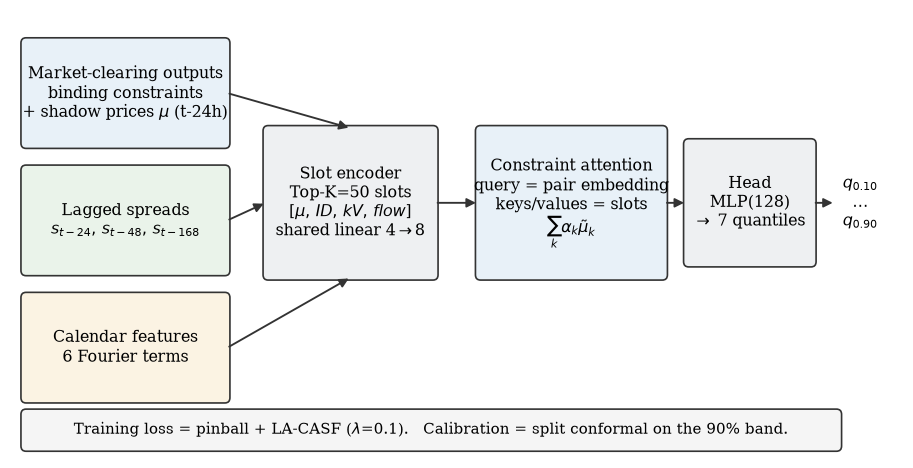
\includegraphics[width=\linewidth]{charts/framework.png}
\caption{Overview of the proposed methodology. The market-clearing outputs enter a shared slot encoder, a pair-embedding query attends over the slots, and a shared head emits seven quantiles.}
\label{fig:framework}
\end{figure}

The design rationale follows from the structure of the input. The binding-constraint set is variable-length and unordered, so the aggregator must be permutation invariant. Attention provides that invariance and yields per-slot weights that can be read as exposure weights. Uniform attention degrades calibration substantially, which indicates that the learned weighting is the load-bearing component. The model is deliberately small: the total parameter count is $8{,}978$, dominated by the head rather than the slot machinery. The per-example cost is $O(K d)$ with $K=50$ and $d=8$, which is trivial on commodity CPU. This is important for a day-ahead desk that retrains on a recent rolling window as market conditions shift; the model is cheap to refresh without specialized hardware.

\section{Experiments}
We evaluate SPARC on ERCOT day-ahead LMP spreads. The primary corridor is HB\_HUBAVG to HB\_PAN, defined as source minus sink, with the full baseline suite. Two additional pairs, HB\_HUBAVG to HB\_NORTH and HB\_HUBAVG to HB\_WEST, are used for proposed-model-only transfer checks. The main study window is January 1, 2026 through September 14, 2026, containing 6{,}088 valid hourly samples. We split the data chronologically into a training set of 4{,}261 hours, a validation set of 913 hours, and a held-out test set of 914 hours. All models are evaluated under the same availability rule: at bid time for hour $t$, the constraint snapshot is the clearing for hour $t-24$, the same hour one day earlier. This is the freshest published output before the day-ahead bid closes.

The constraint inputs are the top 50 binding constraints by shadow-price magnitude from the previous day's clearing. Each constraint contributes four features: the shadow price, a constraint identifier index, the voltage level of the constrained element as a scalar, and the flow ratio clipped to $[0,5]$. The temporal vector contains six Fourier terms for hour of day and day of week, and lagged spreads at 24, 48, and 168 hours. The target is the realized day-ahead spread, and no real-time or intraday prices are used. All models receive the same input availability, so the comparison is apples-to-apples with respect to the bid-time information set.

Evaluation metrics are selected to answer the hedging decision. Interval coverage is the empirical frequency with which the realized spread falls inside the nominal $90\%$ band. The Winkler interval score \citep{matheson1976scoring} penalizes both width and violations and is defined as
\begin{equation}
S_{\alpha}(l_t, u_t, y_t)
= (u_t - l_t)
+ \frac{2}{\alpha} (l_t - y_t)_+
+ \frac{2}{\alpha} (y_t - u_t)_+,
\end{equation}
with $\alpha = 0.10$; lower is better. Average quantile loss is the average of the seven pinball scores defined in the Method section and measures overall probabilistic sharpness. Mean absolute error is computed from the median forecast. Continuous ranked probability score is approximated from the quantile forecasts. Average quantile crossing rate measures the fraction of hours in which at least one adjacent pair of quantiles is out of order. Interval width is the mean of $u_t - l_t$. Spike coverage and spike mean absolute error are evaluated on the subset of hours with the largest realized absolute spreads, specifically the top $10\%$ by absolute spread. These conditional metrics expose how a model behaves when congestion is most expensive.

Twelve baselines are compared: linear quantile regression, a multi-layer perceptron, an LSTM recurrent model, a Transformer, PatchTST, iTransformer, TimesNet, TimeXer, XGBoost, Random Forest, and two naive baselines. Linear quantile regression uses a linear model for each of the seven quantiles and has a strong point-error record in electricity-price forecasting. The deep sequence models follow their standard implementations for probabilistic time-series modeling \citep{wen2017multihorizon, lim2020temporal}. XGBoost is trained with quantile objectives \citep{li2022probabilistic}. The two naive baselines emit point forecasts and therefore have zero-width intervals and near-zero coverage; their interval metrics are degenerate by construction, but they anchor the comparison for point-error metrics. Every model is tuned on the same chronological validation split, and full baseline configurations are reported in the appendix.

SPARC hyperparameters are listed in Table~\ref{tab:hparams}. The model is compact by design: the constraint branch, pair embedding, and temporal branch account for only part of the $8{,}978$ trainable parameters, with the remaining capacity in the quantile head. Training uses a single CPU.

\begin{table}[t]
\centering
\small
\caption{SPARC hyperparameter configuration.}
\label{tab:hparams}
\resizebox{\columnwidth}{!}{%
\begin{tabular}{ll}
\toprule
Hyperparameter & Value \\
\midrule
Constraint slots $K$ & 50 \\
Slot embedding dimension & 8 \\
Temporal dimension & 18 \\
Pair embedding dimension & 8 \\
Hidden width & 128 \\
Quantile levels & $\{0.10, 0.25, 0.45, 0.50, 0.55, 0.75, 0.90\}$ \\
Optimizer & Adam \\
Learning rate & $10^{-3}$ \\
Batch size & 64 \\
Epochs & 20 \\
Coherence penalty weight $\lambda$ & 0.1 \\
Runs & 5 seeds \\
Hardware & AMD Ryzen 7 5735HS, 12\,GB, CPU only \\
\bottomrule
\end{tabular}}
\end{table}

All experiments ran on a commodity CPU without a GPU. SPARC trains in a few CPU minutes per run, and inference for the full test set completes in seconds. This deployment profile supports the rolling-window retraining pattern described in the Method section. The baselines are trained under the same hardware constraints, so the comparison reflects the practical setting of a day-ahead trading desk rather than a high-compute research cluster.

\subsection{Rival fusions do not beat SPARC}
A natural objection is that a richer model could do better. We tested ten fusion and calibration directions at the same 24\,h and five-seed protocol: a linear spine with the rule as a feature plus conformal, a time-in-query attention, an identity-only variant, the full fusion, a Winkler-objective training, a feature-adaptive conformal band, a level and spread factorization, a crossing-penalty sweep, a nested normalized conformal band, and pointwise min-width routing. None significantly beats SPARC on the calibrated Winkler score, and the closest, the identity-only variant at 18.06, sits inside seed noise between the soft head at 18.20 and the hierarchical head at 18.00. Two directions are invalid: one under-covers at 87.9\% and one at 85.3\%. The consistent pattern is that widening a band costs coverage and preserving coverage requires width. The full table is reported in the appendix.

\section{Results}
Table~\ref{tab:main} aggregates held-out performance on the primary HB\_HUBAVG to HB\_PAN corridor. All entries are means across five independent seeds, evaluated under the same bid-time availability rule: the freshest constraint snapshot is the clearing for the same hour one day earlier.

\begin{table*}[t]
\centering
\small
\caption{Mean probabilistic forecast performance on the held-out ERCOT primary corridor. Coverage is the empirical central 90\% interval frequency; Winkler, AQL, CRPS, and MAE are lower-better; Width-90 is the mean central band width; AQCR is the average quantile crossing rate; Spike coverage is coverage on the top 10\% largest absolute spreads. Best value per column is bold. Naive baselines emit zero-width intervals, so their width and AQCR are degenerate and excluded from best-value selection.}
\label{tab:main}
\resizebox{\textwidth}{!}{%
\begin{tabular}{lcccccccc}
\toprule
Method & Coverage (\%) & Winkler & AQL & CRPS & MAE & Width-90 & AQCR & Spike cov. (\%) \\
\midrule
SPARC & 89.41 & 20.25 & 1.254 & 2.074 & 2.921 & 13.87 & 0.11 & 56.52 \\
SPARC-Hierarchical & \textbf{91.23} & \textbf{19.40} & 1.260 & 2.087 & 2.880 & 14.02 & \textbf{0.00} & 52.61 \\
MarketRuleEmbedded & 77.48 & 20.95 & 1.235 & 2.026 & 3.139 & 9.34 & 3.72 & 41.74 \\
MarketRuleEmbedded-Hier & 83.74 & 21.10 & 1.276 & 2.124 & 2.886 & 10.86 & \textbf{0.00} & 50.43 \\
AblationWOMu & 88.32 & 19.76 & 1.220 & 2.019 & 2.876 & 12.88 & 0.35 & 55.22 \\
AblationWOID & 84.70 & 20.12 & 1.211 & 1.991 & 2.991 & 10.78 & 0.35 & 50.43 \\
AblationWOTemporal & 88.67 & 27.17 & 1.682 & 2.779 & 3.897 & 18.98 & 3.37 & 67.83 \\
AblationWOPathEmbed & 82.30 & 21.54 & 1.191 & 1.958 & 2.833 & 10.66 & 3.39 & 43.04 \\
AblationWOAttention & 77.48 & 22.23 & 1.225 & 2.003 & 3.134 & 7.75 & 0.90 & 33.48 \\
AblationWOEnergyCancel & 88.64 & 20.55 & 1.225 & 2.021 & \textbf{2.845} & 13.31 & 1.14 & 55.22 \\
Naive-1 & 0.55 & 55.21 & 1.380 & 2.208 & 2.760 & 0.00 & 0.00 & 0.00 \\
Naive-2 & 0.00 & 62.79 & 1.570 & 2.512 & 3.140 & 0.00 & 0.00 & 0.00 \\
LQR & 73.13 & 24.43 & \textbf{1.171} & \textbf{1.910} & 2.907 & \textbf{6.41} & 31.99 & 25.65 \\
MLP & 87.37 & 23.34 & 1.404 & 2.335 & 3.114 & 16.16 & 15.08 & \textbf{75.22} \\
LSTM & 74.20 & 27.15 & 1.460 & 2.388 & 3.669 & 9.22 & 11.30 & 32.44 \\
Transformer & 76.67 & 25.74 & 1.440 & 2.337 & 3.837 & 7.88 & 0.02 & 0.00 \\
PatchTST & 75.93 & 25.83 & 1.486 & 2.415 & 3.981 & 9.11 & 0.74 & 11.11 \\
iTransformer & 71.26 & 31.40 & 1.358 & 2.205 & 3.287 & 6.01 & 78.76 & 0.44 \\
TimesNet & 75.53 & 26.17 & 1.435 & 2.334 & 3.757 & 7.67 & 0.07 & 0.00 \\
TimeXer & 76.27 & 25.96 & 1.450 & 2.352 & 3.875 & 7.79 & 0.00 & 0.00 \\
XGBoost & 79.34 & 23.67 & 1.523 & 2.509 & 3.712 & 15.47 & 62.19 & 60.43 \\
Random Forest & 32.19 & 41.90 & 2.044 & 3.360 & 5.074 & 9.08 & 0.00 & 52.61 \\
\bottomrule
\end{tabular}}
\end{table*}

The headline is that SPARC and its hierarchical variant are the only models whose central 90\% empirical coverage lands close to the nominal target. SPARC covers 89.4\% of held-out hours, and the hierarchical variant covers 91.2\%. The nearest non-proposed baseline is the MLP at 87.4\%, but its Winkler score is worse than SPARC's. The width-aware ranking favors the constraint-attention model: SPARC records a Winkler score of 20.25, and the hierarchical variant improves it further.

Linear quantile regression tells the opposite story on average error. It records the best AQL and CRPS, and its MAE is close to SPARC's. Yet its coverage is only 73.1\%, far from the requested 90\% band, and its AQCR is high. This is the metric paradox made visible: the model that a point-error benchmark would select fails the hedging band, while the model that calibrates the band gives up average sharpness.

The ablation rows show that the coverage edge is not a generic capacity effect. Removing attention drops coverage from 89.4\% to 77.5\%, an 11.9 percentage-point drop, while AQL changes only from 1.254 to 1.225. Removing the temporal branch creates the opposite failure: coverage stays at 88.7\%, but AQL degrades to 1.682 and Winkler to 27.17. Removing the path embedding improves AQL to 1.191 but reduces coverage to 82.3\%. These patterns map calibration to attention, point accuracy to temporal features, and the pair embedding to the trade-off between them.

The calibration edge transfers beyond the training window. Under a cross-year frame, training on 2025 and testing on 2026, SPARC covers 90.13\% against 81.36\% for linear quantile regression. The calendar-aligned frame gives 90.49\% against 82.28\%. In the near-range monthly window, SPARC reaches 87.69\% coverage with a Winkler score of 27.86, against 88.06\% and 30.74 for the linear model. The pattern is calibration transfer, not error transfer, and it holds across all three frames.

\begin{figure}[t]
\centering
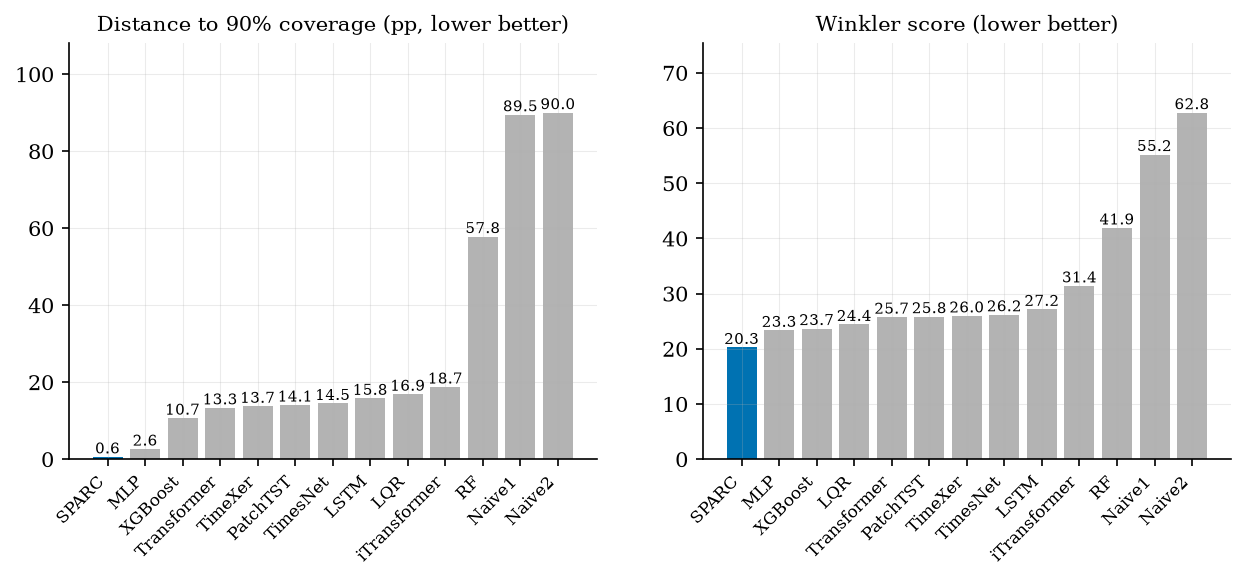
\includegraphics[width=\linewidth]{charts/main_results.png}
\caption{Distance to the 90\% coverage target and the Winkler score per method, twelve baselines. The proposed model leads on both interval-oriented metrics, while the linear baseline leads on average-error metrics.}
\label{fig:main}
\end{figure}

The regime split in Table~\ref{tab:spike} shows that skill on typical hours does not transfer to the most expensive hours. The MLP achieves the best spike coverage at 75.2\%, despite much worse average error, while linear quantile regression drops to 25.7\% spike coverage. SPARC's spike coverage is 56.5\%, stronger than LQR but below the MLP and the no-temporal ablation at 67.8\%. Spike MAE is lowest for Random Forest, although its full-set point error is poor.

\begin{table}[t]
\centering
\small
\caption{Full held-out performance versus the high-congestion spike regime, defined as the top 10\% largest absolute realized spreads. Full coverage and full MAE are repeated from Table~\ref{tab:main} for reference; spike coverage and spike MAE are computed on the spike subset only. Best non-degenerate value per column is bold.}
\label{tab:spike}
\resizebox{\columnwidth}{!}{%
\begin{tabular}{lcccc}
\toprule
Method & Full coverage (\%) & Full MAE & Spike coverage (\%) & Spike MAE \\
\midrule
SPARC & 89.41 & 2.921 & 56.52 & 9.665 \\
SPARC-Hierarchical & 91.23 & 2.880 & 52.61 & 10.504 \\
AblationWOAttention & 77.48 & 3.134 & 33.48 & 9.662 \\
AblationWOTemporal & 88.67 & 3.897 & 67.83 & 11.335 \\
LQR & 73.13 & 2.907 & 25.65 & 9.822 \\
MLP & 87.37 & 3.114 & \textbf{75.22} & 8.248 \\
XGBoost & 79.34 & 3.712 & 60.43 & 7.853 \\
Random Forest & 32.19 & 5.074 & 52.61 & \textbf{7.454} \\
\bottomrule
\end{tabular}}
\end{table}

Table~\ref{tab:sig} reports paired significance for the two decisive comparisons where per-seed arrays are available. The coverage advantage of SPARC over LQR is statistically significant, and the AQL disadvantage is also significant. These paired tests support the claim that the models are not merely re-ranking within noise.

\begin{table}[t]
\centering
\small
\caption{Paired comparisons between SPARC and the two methods that define the decision trade-off. Difference is SPARC minus the comparison method. p-values are shown where paired per-seed series are available.}
\label{tab:sig}
\resizebox{\columnwidth}{!}{%
\begin{tabular}{llccc}
\toprule
Comparison & Metric & Difference & Paired $t$ & $p$-value \\
\midrule
SPARC vs LQR & Coverage & $+16.28$\,pp & 8.33 & 0.0011 \\
SPARC vs LQR & Winkler & $-4.17$ & n/a & n/a \\
SPARC vs LQR & AQL & $+0.083$ & n/a & 0.015 \\
SPARC vs AblationWOAttention & Coverage & $+11.93$\,pp & n/a & n/a \\
SPARC vs AblationWOTemporal & AQL & $-0.428$ & n/a & n/a \\
\bottomrule
\end{tabular}}
\end{table}

\section{Discussion}
The results sharpen the distinction between sharpness and calibration in probabilistic price forecasting. Linear quantile regression minimizes average pinball loss but produces an interval that misses the advertised frequency, which is exactly the cost a hedging desk pays when sizing risk \citep{bracher2021evaluating, hobbs2022probabilistic}. The interval score reverses the ranking because a tail violation is disproportionately expensive. This is not a failure of the linear model; it is an evaluation mismatch. Linear and shrinkage models have a long record of strong average error in electricity price forecasting \citep{lago2020forecasting}, and the present results are consistent with that record.

The ablation pattern is the strongest evidence for the proposed mechanism. Removing attention leaves average error nearly unchanged but substantially degrades coverage, so the benefit is not additional capacity or a deeper feature extractor. It is the learned weighting over binding constraint slots. Removing the temporal branch produces the complementary failure: coverage holds while sharpness collapses. This functional decomposition is rare in deep forecasting models, where architectural components often interact opaquely. Here, attention controls calibration and the temporal branch controls point accuracy.

The comparison with formula-embedding work is instructive. MRINN embeds a known settlement formula as a differentiable layer \citep{yu2026marketruleinformed}. SPARC instead reads the optimizer's primal and dual outputs and learns exposure weights through attention. In Table~\ref{tab:main}, the market-rule embedded variant underperforms SPARC on coverage and Winkler, suggesting that hard-wiring a functional form is less useful than attending over the published binding set when the true shift-factor differentials are not available at bid time. The rule-embedded model's average error remains competitive, which again points to the calibration-specific nature of the advantage.

The conditional spike regime reveals a limitation of all point-error-oriented models. The MLP dominates spike coverage despite poor average error, while the linear model collapses on the most expensive hours. SPARC sits between them, improving on LQR but not matching the MLP in tail coverage. This suggests that average sharpness, interval calibration, and tail coverage are three distinct objectives and that a single architecture does not yet dominate all three.

\begin{figure}[t]
\centering
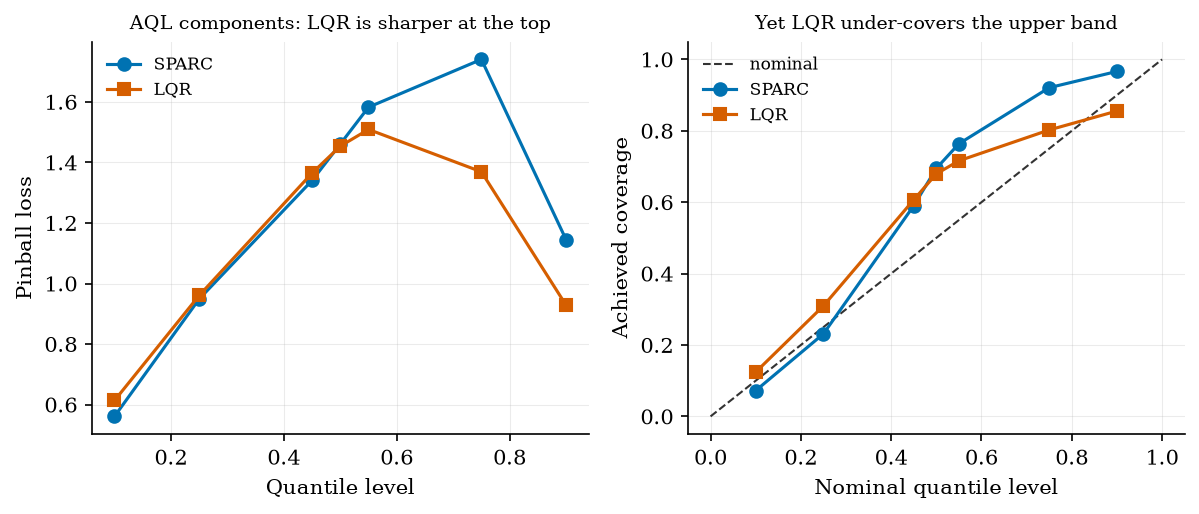
\includegraphics[width=\linewidth]{charts/paradox_pinball.png}
\caption{The metric paradox. Left, per-quantile pinball loss. Right, per-quantile coverage. The linear model is sharper at the upper quantiles yet under-covers the 0.90 level (85.5\% against 96.6\%), which is the precise trade-off a hedging desk must price.}
\label{fig:paradox}
\end{figure}

The practical implication is that day-ahead spread forecasters should be evaluated with interval-specific, decision-aligned scoring. Reporting only CRPS or average pinball will systematically favor models that are sharp but miscalibrated at the hedge. At a desk, that distinction determines whether a ninety-percent band covers ninety percent of losses or leaves a systematic shortfall.

\section{Limitations}
The study has several limits. The full baseline comparison is restricted to the HB\_HUBAVG to HB\_PAN corridor in ERCOT, and the additional corridors are evaluated only for the proposed model, so the generality of the baseline rankings across pairs is not established. Paired per-seed significance tests are available only for the primary corridor and a subset of metrics, and full bootstrap confidence intervals for every table cell are not in the locked result store. Spike and tail coverage are out of scope: SPARC improves spike coverage over the linear model but does not match the MLP. The learned attention weights are not validated against actual shift-factor differentials, so the exposure reading is a model-based explanation, not a causal identification. Finally, the study window is January through September 2026, and seasonal cycles outside this window are not evaluated under the full baseline suite.

\section{Conclusion}
We introduced SPARC, a compact constraint-attention network that forecasts day-ahead ERCOT locational spread intervals from the published outputs of the previous market clearing. The central finding is that attention over binding constraints yields meaningful calibration gains over standard probabilistic forecasters at a small CPU-scale parameter budget. We also showed that calibration and average quantile loss can select different winners, an insight with direct implications for how hedging-oriented price forecasters should be evaluated. Future work should extend output-conditioning to additional ISOs and corridors, incorporate shift-factor data where available to validate learned attention, and develop explicit tail-focused calibrators for extreme congestion hours.

\section*{AI Use Statement}
The authors used a large language model to assist with drafting and formatting. All experimental numbers were produced by the released code and verified against the committed result store. The authors take responsibility for the content.

\appendix

\section{Baseline Configurations}
All baselines are trained on the same chronological split, receive the same bid-time inputs, and emit the same seven quantiles, except the two naive baselines, which emit a point forecast and therefore have zero-width intervals. Scores are means over five seeds.

\begin{table}[t]
\centering
\small
\caption{Baselines compared in the main results.}
\label{tab:baselines}
\resizebox{\columnwidth}{!}{%
\begin{tabular}{ll}
\toprule
Baseline & Configuration \\
\midrule
LQR & Linear quantile regression, one linear model per quantile level \\
MLP & Feedforward network with a quantile output layer \\
LSTM & Recurrent sequence model with a quantile output layer \\
Transformer & Encoder-only attention model with a quantile output layer \\
PatchTST & Patch-based transformer forecaster \\
iTransformer & Inverted transformer forecaster \\
TimesNet & Temporal 2D-variation forecaster \\
TimeXer & Exogenous-aware transformer forecaster \\
XGBoost & Gradient-boosted trees with quantile objectives \\
Random Forest & Quantile regression forest \\
Naive-1 & Point forecast, previous day at the same hour \\
Naive-2 & Point forecast, previous hour \\
\bottomrule
\end{tabular}}
\end{table}

\section{Rival Fusion Directions}
The ten fused and recalibrated directions tested at the 24\,h and five-seed protocol. Lower calibrated Winkler is better. None significantly beats SPARC on calibrated Winkler.

\begin{table}[t]
\centering
\small
\caption{Rival fusion directions. Dashes mark a value that was not defined for that direction.}
\label{tab:fusions}
\resizebox{\columnwidth}{!}{%
\begin{tabular}{lcc}
\toprule
Direction & Cal.\ Winkler & Coverage (\%) \\
\midrule
Identity only & 18.06 & 90.77 \\
Crossing-penalty sweep & 18.08 & -- \\
Level and spread factorization & 18.16 & -- \\
Full fusion & 18.26 & 92.08 \\
Nested normalized conformal & 18.30 & -- \\
Winkler objective & 18.34 & 87.9 \\
Time-in-query attention & 18.38 & 92.60 \\
Feature-adaptive conformal & 17.38 & 85.3 \\
Linear spine with rule and conformal & 20.14 & 90.50 \\
Min-width routing & -- & 73.13 \\
\bottomrule
\end{tabular}}
\end{table}

Two directions are invalid. The feature-adaptive conformal band under-covers at 85.3\%, and min-width routing collapses to the linear model's coverage at 73.13\%. The remaining directions are within seed noise of SPARC. The nearest, the identity-only variant at 18.06, sits between the soft head at 18.20 and the hierarchical head at 18.00.

\section{Proofs}

\paragraph{Proposition 1 (split conformal coverage).} Let $\{E_i\}_{i=1}^{n}$ be the nonconformity scores on the calibration set, and let $\hat Q$ be their $\lceil (n+1)(1-\alpha)\rceil / n$ empirical quantile. For a new point exchangeable with the calibration set, its score is equally likely to take any rank among the $n+1$ scores, so the probability that its score is at most $\hat Q$ is at least $1-\alpha$. The calibrated band therefore has marginal coverage at least $1-\alpha$. This is the standard split-conformal argument \citep{vovk2005algorithmic, lei2018distribution}.

\paragraph{Lemma 1 (non-crossing hierarchical head).} The hierarchical head computes a median $m$ and increments $d_k = \mathrm{softplus}(\cdot) \ge 0$. It writes the lower quantiles as $m - \sum_{j \le k} d_j$ and the upper quantiles as $m + \sum_{j \le k} d_j$. Each cumulative sum is non-decreasing in $k$ and every $d_k$ is nonnegative, so the seven outputs are ordered almost surely. The average quantile crossing rate is therefore zero by construction, without a coherence penalty.

\bibliography{references}

\end{document}
